\section{Características do círculo}

\begin{frame}[fragile]{A constante $\pi$}

    \begin{itemize}
        \item Tanto o cálculo do perímetro quanto da área de um círculo envolvem o uso da 
            constante $\pi$
        \pause

        \item Caso o problema não informe o valor a ser utilizado, há três maneiras de proceder 
            para determinar o valor desta constante
        \pause

        \item A primeira é utilizar o valor definido na linguagem Python, que pode ser obtido com 
            o script abaixo:

        \inputcode{py}{pi.py}
        \pause

        \item O valor resultante, 3.141592653589793, está correto nas suas 15 casas decimais
        \pause

        \item A segunda forma é utilizar a expressão \code{c}{acos(-1.0)} em C/C++
        \pause

        \item A terceira é usar a macro \code{c}{M_PI} da biblioteca de matemática padrão do
            C/C++
    \end{itemize}

\end{frame}

\begin{frame}[fragile]{Perímetro do círculo}

    \begin{itemize}
        \item O perímetro (circunferência) $C$ de um círculo corresponde ao comprimento do contorno do círculo 
        \pause

        \item Este valor pode ser computado como o perímetro de um polígono regular de $n$ lados e
            raio circunscrito $r$ (distância do centro a um dos vértices do polígono), 
            quando $n$ tende a infinito
        \pause

        \item O lado $L$ de tal polígono e o raio se relacionam de modo que
        \[
            \sin \frac{\pi}{n} = \frac{L/2}{r} 
        \]
        \pause

        \item Assim,
        \[
            C = \lim_{n \to \infty} nL
            = \lim_{n \to \infty} n\left(2r\sin \frac{\pi}{n}\right) 
            = 2r \left(\lim_{n \to \infty} n\sin \frac{\pi}{n}\right)
            = 2\pi r
        \]

    \end{itemize}

\end{frame}

\begin{frame}[fragile]{Implementação do perímetro em C/C++}

    \inputcode{cpp}{codes/perimeter.cpp}

\end{frame}

\begin{frame}[fragile]{Área do círculo}

    \begin{itemize}
        \item De modo semelhante, a área $A$ de um círculo pode ser aproximada pela área de um
            polígono regular de $n$ lados e raio circunscrito $r$ quando $n$ tende ao infinito
        \pause

        \item A base de cada triângulo interno é igual a $L$
        \pause

        \item A altura é a apótema $a$, onde
        \[
            \cos \frac{\pi}{n} = \frac{a}{r}
        \]
        \pause

        \item Assim,
        \[
            A = \lim_{n\to \infty} n \left(\frac{La}{2}\right)
            = \lim_{n\to \infty} n \left(r\sin \frac{\pi}{n}\right)\left(r\cos\frac{\pi}{n}\right),
        \] isto é,
        \[
            A = r^2\left(\lim_{n\to\infty} n\sin \frac{\pi}{n}\cos\frac{\pi}{n}\right)
            = r^2\lim_{n\to\infty} n\left(\frac{\sin \frac{2\pi}{n}}{2}\right)
            = \pi r^2
        \]

    \end{itemize}

\end{frame}

\begin{frame}[fragile]{Implementação da área do círculo em C++}
    \inputcode{cpp}{codes/area.cpp}
\end{frame}

\begin{frame}[fragile]{Arcos}

    \begin{itemize}
        \item Um arco de um círculo corresponde a uma seção conectada da circunferência 
        \pause

        \item O comprimento do arco pode ser determinado através do ângulo central $\theta$, 
            definido pelos vetores gerados pela união de cada um dos pontos extremos do arco com
            o centro do círculo
        \pause

        \item Um ângulo de $2\pi$ gera um arco igual a circunferência, isto é, $2\pi r$
        \pause

        \item Usando a proporcionalidade e a regra de três, um ângulo $\theta$  corresponde a um
            arco igual a $\theta r$
        \pause

        \begin{figure}
            \centering
            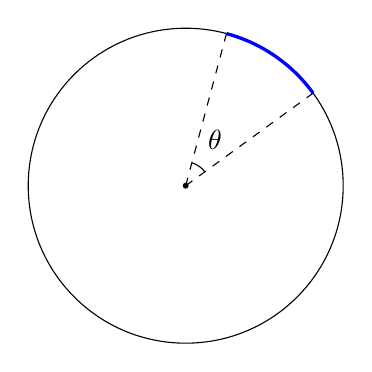
\begin{tikzpicture}
                \draw[fill] (0, 0) circle (0.03cm);
                \draw (0, 0) circle (2);
                \draw[dashed] (0, 0) -- ({2*cos(75)}, {2*sin(75)});
                \draw[dashed] (0, 0) -- ({2*cos(36)}, {2*sin(36)});

                \draw[very thick,blue] ({2*cos(36)}, {2*sin(36)}) arc (36:75:2);
                \draw({0.3*cos(36)}, {0.3*sin(36)}) arc (36:75:0.3);

                \node[anchor=south] at ({0.5*cos(42)}, {0.5*sin(42)}) {$\theta$};

            \end{tikzpicture}
        \end{figure}
    \end{itemize}

\end{frame}

\begin{frame}[fragile]{Implementação do arco de um círculo em C/C++}
    \inputcode{cpp}{codes/arc.cpp}
\end{frame}

\begin{frame}[fragile]{Corda de um círculo}

    \begin{itemize}
        \item Uma corda corresponde a qualquer segmento de reta cujos pontos extremos estão sob o círculo
        \pause

        \item O diâmetro é a maior dentre todas as cordas possíveis de um círculo, e tem
            comprimento $d = 2r$
        \pause

        \item Conhecidos o raio $r$ e o ângulo central $\theta$ do arco definido pela corda, 
            o comprimento $L$ da corda pode ser determinado através da Lei dos Cossenos 
        \[
            L = \sqrt{ 2r^2(1 - \cos\theta)}
        \]
        ou pela Trigonometria
        \[
            L = 2r\sin(\theta/2)
        \]

        \begin{figure}
            \centering
            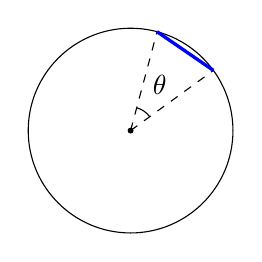
\begin{tikzpicture}
                \draw[fill] (0, 0) circle (0.03cm);
                \draw (0, 0) circle (1.3);
                \draw[dashed] (0, 0) -- ({1.3*cos(75)}, {1.3*sin(75)});
                \draw[dashed] (0, 0) -- ({1.3*cos(36)}, {1.3*sin(36)});

                \draw[very thick,blue] ({1.3*cos(75)}, {1.3*sin(75)}) -- ({1.3*cos(36)}, {1.3*sin(36)});


                \draw({0.3*cos(36)}, {0.3*sin(36)}) arc (36:75:0.3);

                \node[anchor=south] at ({0.5*cos(42)}, {0.5*sin(42)}) {$\theta$};

            \end{tikzpicture}
        \end{figure}
    \end{itemize}

\end{frame}

\begin{frame}[fragile]{Implementação do comprimento de uma corda de um círculo em C/C++}
    \inputcode{cpp}{codes/chord.cpp}
\end{frame}

\begin{frame}[fragile]{Setores}

    \begin{itemize}
        \item Um setor de um círculo é a área delimitada por um arco cujo ângulo central é
            $\theta$
        \pause

        \item Assim como no caso do arco, a área do setor será a fração da área total 
            correspondente ao ângulo central $\theta$ do arco que delimita o setor
        \pause

        \item Assim, a área $S$ do setor é dada por
        \[
            S = \frac{\theta r^2}{2}
        \]
        \pause

        \begin{figure}
            \centering
            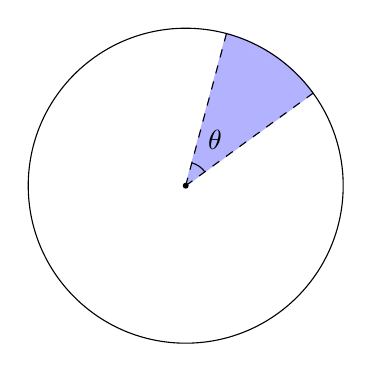
\begin{tikzpicture}
                \draw[fill,blue!30] ({2*cos(36)}, {2*sin(36)}) arc (36:75:2);
                \draw[fill,blue!30] ({2*cos(36)}, {2*sin(36)}) --
                    (0, 0) -- ({2*cos(75)}, {2*sin(75)}) -- ({2*cos(36)}, {2*sin(36)});

                \draw[fill] (0, 0) circle (0.03cm);

                \draw (0, 0) circle (2);
                \draw[dashed] (0, 0) -- ({2*cos(75)}, {2*sin(75)});
                \draw[dashed] (0, 0) -- ({2*cos(36)}, {2*sin(36)});

                \draw({0.3*cos(36)}, {0.3*sin(36)}) arc (36:75:0.3);

                \node[anchor=south] at ({0.5*cos(42)}, {0.5*sin(42)}) {$\theta$};

            \end{tikzpicture}
        \end{figure}
 
    \end{itemize}

\end{frame}

\begin{frame}[fragile]{Implementação do setor de um círculo em C++}
    \inputcode{cpp}{codes/sector.cpp}
\end{frame}

\begin{frame}[fragile]{Segmento}

    \begin{itemize}
        \item Um segmento de um círculo associado a um ângulo central $\theta$ corresponde à área 
            resultante da diferença entre o setor delimitado por $\theta$ e do triângulo 
            resultante do segmentos de reta que unem os extremos dos arcos ao centro do círculo e 
            os extremos entre si (a corda)
        \pause

        \item A área $T$ deste triângulo pode ser determinada pela Fórmula de Heron
        \[
            T = \sqrt{s(s - r)(s - r)(s - c)},
        \] onde $s$ é o semiperímetro, dado por
        \[
            s = \frac{2r + c}{2}
        \] e $c$ o comprimento da corda, isto é
        \[
            c = 2r\sin(\theta/2)
        \]
    \end{itemize}

\end{frame}

\begin{frame}[fragile]{Visualização do segmento de um círculo}

    \begin{figure}
        \centering
        \begin{tikzpicture}
            \draw[fill,blue!30] ({3.7*cos(36)}, {3.7*sin(36)}) arc (36:75:3.7);

            \draw[fill] (0, 0) circle (0.03cm);

            \draw (0, 0) circle (3.7);
            \draw[dashed] (0, 0) -- ({3.7*cos(75)}, {3.7*sin(75)});
            \draw[dashed] (0, 0) -- ({3.7*cos(36)}, {3.7*sin(36)});

            \draw({0.3*cos(36)}, {0.3*sin(36)}) arc (36:75:0.3);

            \node[anchor=south] at ({0.5*cos(42)}, {0.5*sin(42)}) {$\theta$};

        \end{tikzpicture}
    \end{figure}

\end{frame}

\begin{frame}[fragile]{Implementação do segmento de um círculo em C/C++}
    \inputcode{cpp}{codes/segment.cpp}
\end{frame}
